%% The first command in your LaTeX source must be the \documentclass command.
%%%% Small single column format, used for CIE, CSUR, DTRAP, JACM, JDIQ, JEA, JERIC, JETC, PACMCGIT, TAAS, TACCESS, TACO, TALG, TALLIP (formerly TALIP), TCPS, TDSCI, TEAC, TECS, TELO, THRI, TIIS, TIOT, TISSEC, TIST, TKDD, TMIS, TOCE, TOCHI, TOCL, TOCS, TOCT, TODAES, TODS, TOIS, TOIT, TOMACS, TOMM (formerly TOMCCAP), TOMPECS, TOMS, TOPC, TOPLAS, TOPS, TOS, TOSEM, TOSN, TQC, TRETS, TSAS, TSC, TSLP, TWEB.
% \documentclass[acmsmall]{acmart}

%%%% Large single column format, used for IMWUT, JOCCH, PACMPL, POMACS, TAP, PACMHCI
%\documentclass[acmlarge,screen]{acmart}

%%%% Large double column format, used for TOG
%\documentclass[acmtog, authorversion]{acmart}

%%%% Generic manuscript mode, required for submission
%%%% and peer review
%\documentclass[sigconf, anonymous]{acmart}
\documentclass[manuscript,screen,review,anonymous,acmsmall]{acmart}

\usepackage{csquotes}
\usepackage{soul}

%DIF PREAMBLE EXTENSION ADDED BY LATEXDIFF
%DIF UNDERLINE PREAMBLE %DIF PREAMBLE
\RequirePackage[normalem]{ulem} %DIF PREAMBLE
\RequirePackage{color}\definecolor{RED}{rgb}{1,0,0}\definecolor{BLUE}{rgb}{0,0,1} %DIF PREAMBLE
\providecommand{\DIFadd}[1]{{\protect\color{blue}\uwave{#1}}} %DIF PREAMBLE
\providecommand{\DIFdel}[1]{{\protect\color{red}\sout{#1}}}                      %DIF PREAMBLE
%DIF SAFE PREAMBLE %DIF PREAMBLE
\providecommand{\DIFaddbegin}{} %DIF PREAMBLE
\providecommand{\DIFaddend}{} %DIF PREAMBLE
\providecommand{\DIFdelbegin}{} %DIF PREAMBLE
\providecommand{\DIFdelend}{} %DIF PREAMBLE
%DIF FLOATSAFE PREAMBLE %DIF PREAMBLE
\providecommand{\DIFaddFL}[1]{\DIFadd{#1}} %DIF PREAMBLE
\providecommand{\DIFdelFL}[1]{\DIFdel{#1}} %DIF PREAMBLE
\providecommand{\DIFaddbeginFL}{} %DIF PREAMBLE
\providecommand{\DIFaddendFL}{} %DIF PREAMBLE
\providecommand{\DIFdelbeginFL}{} %DIF PREAMBLE
\providecommand{\DIFdelendFL}{} %DIF PREAMBLE
%DIF END PREAMBLE EXTENSION ADDED BY LATEXDIFF

\newcommand{\NGO}{\textit{NGO}}
\newcommand{\PC}{\textit{GigCo}}
\newcommand{\SRP}{OCP}

%% Rights management information.  This information is sent to you
%% when you complete the rights form.  These commands have SAMPLE
%% values in them; it is your responsibility as an author to replace
%% the commands and values with those provided to you when you
%% complete the rights form.
\setcopyright{rightsretained}
\copyrightyear{2022}
\acmYear{2022}
\acmDOI{10.1145/3532106.3533570}

%% These commands are for a PROCEEDINGS abstract or paper.
\acmConference[ANON '23]{Anon}{Anon, 2023}{Anon}
\acmBooktitle{Anon, 2023}\acmDOI{Anon}
\acmISBN{Anon}


%%
%% Submission ID.
%% Use this when submitting an article to a sponsored event. You'll
%% receive a unique submission ID from the organizers
%% of the event, and this ID should be used as the parameter to this command.
%%\acmSubmissionID{123-A56-BU3}

%%
%% The majority of ACM publications use numbered citations and
%% references.  The command \citestyle{authoryear} switches to the
%% "author year" style.
%%
%% If you are preparing content for an event
%% sponsored by ACM SIGGRAPH, you must use the "author year" style of
%% citations and references.
%% Uncommenting
%% the next command will enable that style.
%%\citestyle{acmauthoryear}

%%
%% end of the preamble, start of the body of the document source.
\begin{document}

% The ontology's name
\newcommand{\ONT}{SIST}

%%
%% The "title" command has an optional parameter,
%% allowing the author to define a "short title" to be used in page headers.
\title{A Design Vocabulary for Scaffolding Group Interaction Archetypes through Synchronous Telephony}

%%
%% The "author" command and its associated commands are used to define
%% the authors and their affiliations.
%% Of note is the shared affiliation of the first two authors, and the
%% "authornote" and "authornotemark" commands
%% used to denote shared contribution to the research.
\author{Dan Richardson}
\email{dan.richardson@monash.edu}
\affiliation{%
  \institution{Monash University}
  \city{Melbourne}
  \country{Australia}}

\author{Md Adnanul Islam}
\email{adnan.islam@monash.edu}
\affiliation{%
  \institution{Monash University}
  \city{Melbourne}
  \country{Australia}}
  
\author{Bronwyn J. Cumbo}
\email{bronwyn.cumbo@monash.edu}
\affiliation{%
  \institution{Monash University}
  \city{Melbourne}
  \country{Australia}}
  
\author{Pranita Shrestha}
\email{pranita.shrestha@monash.edu}
\affiliation{%
  \institution{Monash University}
  \city{Melbourne}
  \country{Australia}}  
  
\author{Delvin Varghese}
\email{delvin.varghese@monash.edu}
\affiliation{%
  \institution{Monash University}
  \city{Melbourne}
  \country{Australia}} 
  
\author{Tom Bartindale}
\email{tom.bartindale@monash.edu}
\affiliation{%
  \institution{Monash University}
  \city{Melbourne}
  \country{Australia}}

\author{Patrick Olivier}
\email{patrick.olivier@monash.edu}
\affiliation{%
  \institution{Monash University}
  \city{Melbourne}
  \country{Australia}}

%%
%% By default, the full list of authors will be used in the page
%% headers. Often, this list is too long, and will overlap
%% other information printed in the page headers. This command allows
%% the author to define a more concise list
%% of authors' names for this purpose.
\renewcommand{\shortauthors}{Anon et al.}

%%
%% The abstract is a short summary of the work to be presented in the
%% article.
\begin{abstract}
Multiple HCI projects have demonstrated the potential of digitally-enhanced, synchronous telephony platforms for use with and by resource-limited communities. However, these platforms were each designed to only facilitate a single archetype of community engagement, limiting their capacity for adaptation when contextual or stakeholder requirements change. This paper builds upon these projects to introduce a design vocabulary, grounded in a formal ontology describing the core components necessary to run adaptable, structured engagements through synchronous group telephony. Through a series of scenarios, we demonstrate how this design vocabulary can be used to: help design and communicate different models of synchronous audio engagements, describe existing technologies, and highlight other novel ways in which such platforms could be used. We discuss how while under-explored to this point, synchronous telephony platforms can be designed to orchestrate stakeholder engagements with a degree of flexibility previously impossible in remote, offline contexts.

% Multiple HCI projects have explored and demonstrated the potential of digitally-enhanced, synchronous telephony platforms for use with and by resource-limited communities. However, these platforms were each designed to only facilitate a single archetype form of community engagement—typically traditional talk shows with some audience interaction—limiting their capacity for adaptation when contextual or stakeholder requirements change. This paper examines the lessons learned from these projects, building upon them and the recent work surrounding object-based media to introduce Paroli: a flexible telephone conferencing system designed to facilitate the scaffolding of new formats of synchronous audio communication. Through a series of use-case scenarios and prototype deployments, we discuss and demonstrate how synchronous telephony platforms can be designed to orchestrate stakeholder engagements with a degree of flexibility previously impossible in remote contexts.
\end{abstract}

%%
%% The code below is generated by the tool at http://dl.acm.org/ccs.cfm.
%% Please copy and paste the code instead of the example below.
%%
\begin{CCSXML}
<ccs2012>
   <concept>
       <concept_id>10003120.10003121.10003122</concept_id>
       <concept_desc>Human-centered computing~HCI design and evaluation methods</concept_desc>
       <concept_significance>500</concept_significance>
       </concept>
   <concept>
       <concept_id>10003120.10003123.10010860.10010859</concept_id>
       <concept_desc>Human-centered computing~User centered design</concept_desc>
       <concept_significance>500</concept_significance>
       </concept>
 </ccs2012>
\end{CCSXML}

\ccsdesc[500]{Human-centered computing~HCI design and evaluation methods}
\ccsdesc[500]{Human-centered computing~User centered design}

%%
%% Keywords. The author(s) should pick words that accurately describe
%% the work being presented. Separate the keywords with commas.
\keywords{IVR, design, resource-limited settings, ICT4D}


%%
%% This command processes the author and affiliation and title
%% information and builds the first part of the formatted document.
\maketitle

\section{Introduction}

The value of technologies which support synchronous remote group communication has been reinforced in recent years, with the increased adoption of remote work, recreation, research, and education \cite{cumbo2021, scriven2021, takashi2012}. However, those technologies are often inaccessible to communities who lack reliable access to digital infrastructure or high levels of literacy \cite{kommiya2019}. Recent HCI research has explored the use of telephony to support resource-limited communities accessing the types of services typically associated with Internet-based infrastructures \cite{khullar2021, Csik2016, Richardson2022, eitzinger2019}. While the majority of these Interactive Voice Response (IVR) platforms enable asynchronous communication (e.g. voice forums for discussion and knowledge sharing \cite{Patel2010}), a recent focus has emerged on the use of telephony to enable synchronous group communication. These technologies have typically been used to infrastructure `broadcast radio' style talk shows with underprivileged communities: supporting listeners with platforms for discussion and access to expert knowledge through audio interfaces, without requiring specialised equipment or Internet access \cite{Kazakos2016, Yadav2017, Talhouk2017}. 

However, while recent research has investigated the repurposing and reconfiguration of Internet-based technologies such as Zoom to adapt to diverse new use cases \cite{Bartindale2021} and to improve perceptions and outcomes of multitasking \cite{marlow2016}, the use of these synchronous telephony platforms beyond these `talk show' formats has been limited: as they are described, each appear to have been built to specifically accommodate a specific engagement structure, without consideration to adaptability or how emergent formats of audio interaction could be supported. The focus on these `single use case' platforms, each designed to facilitate the same interaction archetypes, has meant that communities lacking access to more flexible online synchronous communication platforms such as Zoom are currently excluded from engaging in these emerging forms of remote participation. Furthermore, during the development of our own synchronous telephony platform, we realised that many of these systems are built upon similar technologies and underlying design approaches: we found we were combating a steep learning curve when interfacing with (frequently poorly documented) telephony software stacks, simply to re-tread ground already contributed in prior research projects.

As seen in other emerging HCI design contexts (such as human-IoT system interaction \cite{Chuang2018}, or user identification through touch \cite{Kharrufa2017}), a lack of agreed upon context-independent terminology to describe components, behaviours and characteristics can inhibit designers engaging with the space---especially those who are non-technical \cite{Kharrufa2017}. Similarly, believe that there is a non-trivial barrier to entry for HCI designers and developers entering the space of synchronous telephony: that research has been limited by a lack of a cohesive vocabulary which differentiates between potential design spaces and the underlying technical architecture required to support them. Without this differentiation, subsequent projects have had to `reinvent the telephony wheel' as we did: spending significant development time designing and building (very similar, nonnovel) underlying infrastructures, rather than concentrating on exploring the multiple design spaces these platforms could provide. 

To address this issue, this paper contributes a design vocabulary for synchronous group telephony: a visual framework which, by utilising a concrete set of terms and relationships defined in a formal ontology, is designed to help prototype, communicate and integrate synchronous telephony designs. To illustrate how this vocabulary can assist in designing synchronous telephony platforms, we first demonstrate its application to the established talk show format used in prior research projects. Then, by applying it to other possible use cases, we discuss how such platforms can be designed to orchestrate remote stakeholder engagements with a degree of flexibility previously impossible in contexts with offline participants. We hope that by introducing a cohesive set of axioms and differentiation between interaction design and technical infrastructure, this design vocabulary will support future researchers in identifying and navigating the multiple rich, under-explored design spaces of synchronous group telephony.
\section{Related Work}

\subsection{IVR \& Asynchronous Audio}

By allowing users to interact with digital systems through standard phone calls using their phone's keypad (and sometimes even their voice \cite{khullar2021}), Interactive Voice Response (IVR) systems have been shown to be an effective tool for information retrieval and exchange: especially in low-resource contexts where users have limited internet access \cite{eitzinger2019} and low literacy inhibits the usability of text-based interfaces \cite{sharma2009}. IVR and asynchronous audio has proven to be a versatile medium, with previous projects utilising it in a wide variety of contexts and use cases, including: performing voice-based surveys \cite{khullar2021_surveys}; supporting users in accessing information on-demand \cite{Riaz2017}; connecting offline workers to online marketplaces \cite{Richardson2022}; enabling citizen journalism \cite{Ejaz2018}; creating `voice forums', where users can create and respond to audio messages through phone calls \cite{Patel2010, Vashistha2015}; and interacting with automated conversational agents (`chatbots') to access information \cite{Jain2018, Yadav2019}. These systems offer greater accessibility to users from communities with oral traditions \cite{Ndwe2012}, and can be designed to support cost-free, on-demand access to end-users \cite{Richardson2022}. Additionally, prior studies have highlighted the value of being able to access recordings for later reference on-demand \cite{Talhouk2017}, with the ability to repeatedly access the same information being useful for low-literate users who cannot write information down \cite{Jain2018}. 

Despite the versatility and scalability afforded by this infrastructure, however, automated IVR systems aren't always able to fulfill users' highly specific and contextual queries: traditional IVR menu structures are limited in scope, requiring designers to choose what information and interactions should be prioritised \cite{Richardson2022}. Chatbots have been shown to be able to respond accurately to highly specific queries \cite{Jain2018}, but such systems are dependant on currently unreliable speech-to-text systems and access to extensive databanks of previous responses by human experts. Furthermore, for users unfamiliar with the limitations of chatbots, interacting with them can clash with expectations of interacting with a human over the phone \cite{Jain2018}: resulting in conversational queries which humans could interpret correctly, but automated systems struggle with \cite{Yadav2019}. Meanwhile, voice forums offer human replies, but the ability for anyone to respond to queries can lead to misinformation \cite{Patel2010}, as well as harassment, threats, and systemic marginalisation towards women and minorities \cite{Vashistha2019}.

\subsection{Radio \& Synchronous Audio Platforms}
\label{section:talkshow}

Synchronous voice formats, such as radio, can address these issues through direct moderation of a synchronous activity by a host. Often run by volunteers, community radio stations broadcast live audio content to local communities: offering a method for civic engagement, deliberation and knowledge sharing \cite{Cibin2019, Maye2020}. Projects such as RootIO, a hardware and software platform which supports communities in operating low-cost radio stations, have drastically lowered the costs of radio infrastructure and encourage community-led participatory programming \cite{Csik2016}: particularly when combined with technologies for generating audio content, such as text-to-speech \cite{Scott2020}. Unfortunately, while many radio programmes offer the ability for audiences to call into a show to ask questions, by default radio is an inherently passive medium in terms of audience interaction. Furthermore, broadcast radio often requires the navigation of local policy and broadcast content standards: erecting legal, logistical and psychological barriers due to formal license applications and requirements \cite{Maye2020, Bidwell2021}.

In recent years, researchers such as Kazakos et al. \cite{Kazakos2016} have begun sidestepping these barriers by providing access to `radio' programming through phone-based platforms: hosting live shows through synchronous telephony, with listeners able to dial in with their phones to listen and ask questions to a host controlling the show from a smartphone or web application. These platforms use free, `off the shelf' software such as FreeSWITCH\footnote{\url{https://signalwire.com/freeswitch}} to programmatically manipulate phone calls. 

In these platforms \cite{Kazakos2016, Talhouk2017, Yadav2017}, participants join an engagement by either receiving a phone call or initiating a `callback' (where the system hangs up on incoming calls and immediately calls them back, so that participants aren't charged). Participants spend the majority of the engagement muted, passively listening to one or more unmuted users: a `host' user and, if present, guests (typically experts in their field, e.g. healthcare providers \cite{Talhouk2017}). These discussions are typically unscripted. The engagements often also have a question and answer (Q\&A) segment, where members of the audience can request to be unmuted by pressing a button on their phone. The host can see these requests through a visual interface, and choose who to unmute and when to re-mute them. The audience member's question would then be discussed by the host and/or guests before moving onto the next question. Some platforms also support the recording and playback of audio during the call \cite{Talhouk2017, Yadav2017}.

Yadav et al. note the potential for such platforms to go beyond the `radio' model by additionally supporting asynchronous pre- and post- show interactions, where the audience could dial into the system to submit questions or relisten to prior content on demand \cite{Yadav2017}. As Kazakos et al. (and follow-up investigations by researchers using similar systems \cite{Talhouk2017, Yadav2017}) demonstrate, synchronous telephony allows for remote group engagements with a low barrier to entry, and offers the potential for active audience participation: bringing education, training, and individuals' specific expertise into the homes of rural and underprivileged communities, for whom such knowledge might otherwise have been inaccessible.

Despite this promise, however, these platforms still feature significant design limitations: taken as described in their publications, they are all configured exclusively around the `talk show' concept, with the call host primarily leading discussions with a domain expert and fielding questions from the (otherwise muted) listening audience. These projects have highlighted a number of challenges with this format: for example, a dependence on questions can lead to `content black holes' when they are not received \cite{Kazakos2016}; and while this can be mitigated through pre-prepared audio content \cite{Yadav2017}, an over-reliance on recorded audio and muted participants doesn't take full advantage of the dynamic possibilities of synchronous audio, nor the two-way nature of typical telephone interactions. Furthermore, there is an asymmetrical power imbalance embedded in the talk show design pattern: the call's host has a visual overview and control over the call and its participants, while others---outside of requesting to be unmuted---are relegated to being passive consumers \cite{Varghese2022}. This would make the format unsuitable in contexts which value more open, free-flowing and unbiased discussion \cite{Fiesler2019}, or those that require structured procedure to allow for equal opportunities for participation \cite{robert2020}. Due to the specialisation of these projects and their lack of separation between the concerns of engagement design and core infrastructure, in practice any context which requires an engagement archetype that significantly differs from a talk show necessarily requires the design and implementation of a new, custom-built platform.

\subsection{Ontologies, Design Vocabularies, \& Group Telephony}

Having an agreed-upon terminology to describe the components, behaviours, and characteristics of emerging or underexplored technologies can support the design, development and comparison of implementations of them. Formal ontologies are often produced with this use-case in mind: intended to create `\textit{a shared and common understanding of some domain that can be communicated across people and computers}' \cite{struder1998}, or `\textit{represent elements of the physical world}' \cite{Brubaker2011}. They can be used to create and communicate consensual conceptual models (referred to as `domain reference' ontologies), which can then be further developed to be used to support semantic interoperability within automated systems (referred to as being `operational') \cite{guizzardi2007} when written in a machine-interpretable language such as OWL (Web Ontology Language\footnote{\url{https://www.w3.org/OWL/}}). To support extensibility and reusability, ontologies are frequently organised within three tiers: \textit{foundational}, which describe fundamental concepts that can be shared and reused across many fields (e.g. `a thing'); \textit{core}, which build upon foundational axioms to provide abstract definitions more specific to a particular field (e.g. `a document is a thing'); and \textit{domain}, a definition of concepts and relations concerning a specific, specialised domain (e.g. `a forum post is a document') \cite{scherp2011}. Ontologies have been used to structure and infer knowledge, support reasoning, and serve as a basis for developing systems or frameworks across the HCI and CSCW communities---such as within user interface design, ubiquitous computing, user modeling, design methods, usability, accessibility, and online community collaboration \cite{costa2021, Kamran2016}.

Beyond formal ontologies, other approaches have been used within HCI to describe and illustrate the characteristics of technologies and interactions with them. For example, Kharrufa et al. contributed a conceptual model which allowed for the visual communication of different approaches to user identification on multi-touch devices: aiming to support non-technical practitioners to compare the common parameters that characterize them, independent of their specific use-cases \cite{Kharrufa2017}. Similarly, Chuang et al. produced a `design vocabulary' to describe user-computer communication within IoT systems, supporting the comparison and design of different forms of interaction \cite{Chuang2018}. In comparison to the aforementioned machine-interpretable ontologies which focus on describing existing implementation, these examples instead place greater focus on future design: communicating a system's requirements, strengths, limitations, or possibility space through the use of visuals and hypothesised future technologies. 

\begin{figure}[h]
  \centering
  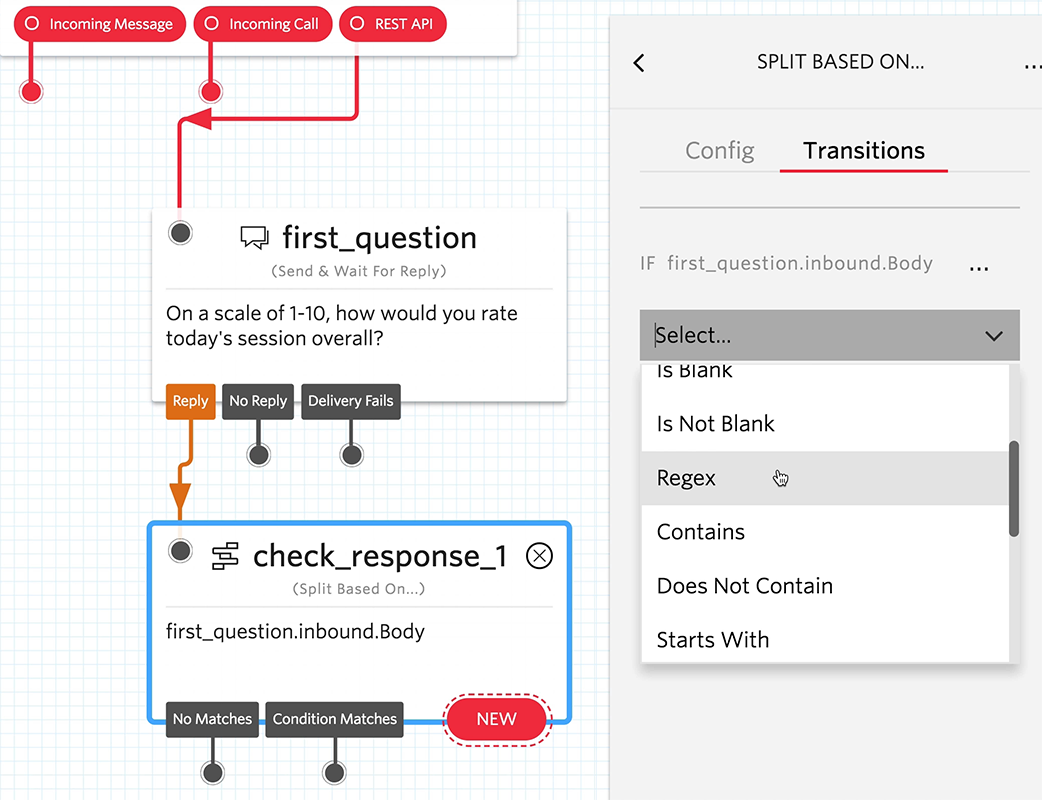
\includegraphics[width=0.6\linewidth]{images/twilio.png}
  \caption{Twilio's Studio interface, which allows for producing IVR logic through a visual programming interface.}
  \Description{A screenshot of Twilio's Studio interface. It shows a GUI in a flow chart style format, with nodes connected by arrows. The first node in the chain is "REST API", and connects with an arrow to a card titled "first question". This card contains the text "on a scale of 1-10, how would you rate today's session overall?". The card has exit nodes titled "Reply", "No Reply", and "Delivery Fails". The "Reply" node is connected by an arrow going to a second card, titled "check_response_1", which is currently being produced by the script author.}
  \label{fig:twilio}
\end{figure}

While prior works have explored the use of ontologies to drive contextual dialogues in IVR systems \cite{ababneh2013, thirumaran2015, thirumaran2015a}, detail the technical aspects of radio transmission and operation \cite{ihmcIHMCOntology}, describe media industry production workflows \cite{movielabs2021}, and support the automatic processing and annotation of meetings \cite{niekrasz2006}, we have not identified an ontology or design vocabulary that describes the configuration and composition of synchronous group interaction archetypes, or how they can be scaffolded or facilitated remotely through telephony. Tools do exist to rapidly develop (and therefore describe) IVR platforms using visual interfaces (e.g. Twilio Studio\footnote{\url{https://www.twilio.com/serverless/studio}}), allowing users to scaffold IVR interactions without requiring significant programming experience through a visual representation of logic (Figure \ref{fig:twilio}). However, these tools largely focus on the design of asynchronous interactions (e.g. SMS surveys, IVR menus) or connecting callers to separately handled synchronous activities (e.g. a helpline), without describing or offering granular controls over synchronous group interactions. As such, there exists a need for a set of agreed upon terms and metaphors to assist designers in conceptualising, visualising, and communicating synchronous group telephony systems and interactions.
\section{Ontology Development}

In response, we set out to develop a vocabulary which could be used by designers and developers as a tool to easily design and communicate different models of synchronous audio engagements, describe existing technologies, and highlight other novel ways in which such platforms could be used. As such, we decided to produce two outputs: a formal ontology called Scaffolding Interactions through Synchronous Telephony (\ONT{}), which would define the terms for the necessary system components and how they interact; and a design vocabulary built upon \ONT{}, supporting less technical stakeholders in exploring potential designs and identifying their strengths, weaknesses and requirements through a visual format reminiscent of Twilio's Studio interface.

Costa et al. argue that following ontology engineering methods tends to result in higher quality ontologies, as they encourage the adoption of best practices and support the identification of user requirements \cite{costa2021}. However, their systematic review of HCI ontologies found that only 3 of the 35 HCI ontologies they analysed were developed using one. Two of these were developed using NeOn: a framework which provides 9 methodology configurations for various use-case scenarios \cite{gomez2009, suarez2012}. These scenarios offer different procedures based on how much the new ontology should reuse or re-engineer existing ontological resources: from generating a new ontology from scratch, to the extension, adaptation, or even localisation of existing ontologies. As this scenario system provides a clear step-by-step methodology, we decided to use NeOn to develop \ONT{}.

As one of the key strengths of formal ontologies is that they can be extended, re-used, and made compatible with each other \cite{scherp2011}, we wanted to build upon existing core concepts: adding our own domain-level axioms relating to synchronous audio engagements on top of existing ontological resources. As such, we decided that NeOn's third scenario, `\textit{Reusing Ontological Resources}', is most suitable for that purpose. Ontologies in this scenario \cite{suarez2012_reuse} should be produced through the following procedure: requirements specification for the new ontology---including its purpose, scope, and intended users---through the generation of competency questions (CQs) and non-functional requirements; reformulating the CQs to support the identification of `linking axioms' in existing ontologies; searching for and identifying ontologies which can fulfill these linking axioms, and then engineering the new ontology through an appropriate development process. This section describes the outputs of each section of this methodology.

\subsection{Requirements Specification}
The key questions of the NeOn requirements specification activity \cite{suarez2012_requirements}, and our responses to them, are as follows: 

\subsubsection{What is the goal of the ontology?}
To describe the key infrastructure and logical components of a platform that supports one or more models of synchronous group telephony, without requiring complete re-engineering for each different engagement format.

\subsubsection{Who are its intended users?}
Software engineers, HCI researchers and designers.

\subsubsection{What are its intended uses?} To support the conceptualisation, visualisation, and communication of synchronous group telephony systems and interactions: to ease the burden of designing and building them and support the exploration of them as a design space.


\subsubsection{What are the requirements it should fulfill?}
 
To respond to this question, we analysed the established design patterns (i.e. the talk show format) and functionality used by previous projects in the space \cite{Kazakos2016, Talhouk2017, Yadav2017}, as discussed in \ref{section:talkshow}. To support the talk show format, these platforms use much of the base functionality made readily available by software such as FreeSWITCH: dialing and disconnecting callers; muting and unmuting individuals; transferring callers into a single `conference' group call; and recording and playing back audio files---either to individuals or everyone on the call. To be of use, these functions need to be mediated by an application with which the host can interact. Our ontology would need to describe these functions, as well as how they could be combined and utilised either programmatically or manually by the host to support various (and even novel, unexplored within this context) engagement formats, without each different format requiring a full platform re-write.

Given the answers to the previous questions, the non-functional requirements for \ONT{} are:

\begin{itemize}
    \item NFR1: The ontology should feature a separation of concerns between the technical infrastructure that supports base phone call functionality, and the application logic that implements activity procedure.
    \item NFR2: The axioms describing these activities should also be able to be configured in a way which can be used to easily design and communicate activity processes in a visually intuitive format.
    \item NFR3: The ontology should feature enough detail and scope to adequately describe the key components of a platform's required architecture and engagements held through it, but not so much to as inhibit design explorations.
\end{itemize}

To determine the functional requirements, NeOn recommends using the prior answers to generate competency questions which the ontology should be able to address, and organising them into categories. For \ONT{}, 56 CQs were developed by the two lead authors. These were then categorised through an inductive card sorting activity into 3 themed groups: `Activity Procedure \& Implementation', `Current State', and `Engagement Data'. A selection of CQs from each group can be seen in Tables \ref{tab:CQ_activity}, \ref{tab:CQ_state}, and \ref{tab:CQ_data}.

\begin{table}
  \caption{Example Competency Questions: Activity Procedure \& Implementation}
  \label{tab:CQ_activity}
  \begin{tabular}{cll}
    \toprule
    CQ\#&Question&Example Response\\
    \midrule
    1&What is the next item in the activity agenda?&Play an audio file\\
    2&What will cause the next procedure to start?&Host presses a button\\
    3&What should happen when participant X presses button 5?&Raise their hand\\
    4&Which participants should be muted?&All except the host\\
    5&What functionality is required to support a pre-show routine?&Play/Stop audio, Mute\\
  \bottomrule
\end{tabular}
\end{table}

\begin{table}
  \caption{Example Competency Questions: Current State}
  \label{tab:CQ_state}
  \begin{tabular}{cll}
    \toprule
    CQ\#&Question&Example Response\\
    \midrule
    6&Which participants are in the call?&List of participants\\
    7&Which participants have their hands raised?&List of participants\\
    8&Which participants are muted?&List of participants\\
    9&Has the host joined the call?&False\\
    10&Which participants are currently speaking?&List of participants\\
  \bottomrule
\end{tabular}
\end{table}

\begin{table}
  \caption{Example Competency Questions: Engagement Data}
  \label{tab:CQ_data}
  \begin{tabular}{cll}
    \toprule
    CQ\#&Question&Example Response\\
    \midrule
    11&When did participant X join the current call?&2023/03/26 14:01\\
    12&Which participants joined the current call, but have left?&List of participants\\
    13&Which participants' questions went unaddressed?&List of participants\\
    14&Where is participant X’s recording stored?&Filepath\\
    15&Which errors occurred during the last engagement?&Badly formatted number\\
  \bottomrule
\end{tabular}
\end{table}

\subsection{Reusing Ontological Resources}

Adapting or expanding upon existing ontological resources can both avoid `reinventing the wheel' \cite{suarez2012} and support extensibility and use alongside other vocabularies within a network \cite{scherp2011}. To select appropriate ontologies, NeOn recommends reformulating the initial competency questions with new, more generic terms `\textit{that could potentially belong to ontologies to be reused}' and to `\textit{identify axioms that link terms of the CQs to terms that could be reused}' \cite{suarez2012_reuse}. Examples of how we adapted our CQs to find more generic terms can be seen in Table \ref{tab:CQ_reformed}. Once some potential axioms were developed, we then searched for ontologies which implemented them, rewording them if unsuccessful (failed alternatives are included in Table \ref{tab:CQ_reformed}). Unfortunately a number of the Semantic Web search engines recommended by the NeOn authors are now offline, however we were able to successfully use a combination of Google and Linked Open Vocabularies\footnote{\url{https://lov.linkeddata.es/dataset/lov}} to find a wide array of popular ontologies. Once a potential axiom had been found, the rest of that ontology was browsed for other matches, or more suitable axioms which had not been thought of during the reformation process.

\begin{table}
  \caption{Example Reformed Competency Questions}
  \label{tab:CQ_reformed}
  \begin{tabular}{p{3.2cm} p{3cm} p{2.8cm} p{3cm} }
    \toprule
    Case&CQ&Action&Result\\
    \midrule
    Want to know the participants in given a group call&Which participants are in the call?&Participants$\rightarrow$ \newline callers/people;\newline Call$\rightarrow$ room/space&Which people are in the space?\\ 
    \midrule
    Want to know the storage location of a participant's recording&Where is participant X’s recording stored?&Where$\rightarrow$ space/location\newline Recording$\rightarrow$ file/data/document&In what space is user X’s document stored?\\ 
    \midrule
    Want to know the next item to be active in the activity procedure&What is the next item in the activity agenda?&Agenda$\rightarrow$\newline list/plan/container&What is the next item in the container?\\ 
  \bottomrule
\end{tabular}
\end{table}


Two existing ontologies were found to be particularly suitable: Friend of a Friend (aka `\textit{foaf}': an ontology describing people, their activities and their relations to other people and objects\footnote{\url{http://xmlns.com/foaf/0.1/}}) and Semantically Interlinked Online Communities (aka `\textit{sioc}': an ontology which builds on \textit{foaf} to describe online community spaces, such as forums\footnote{\url{http://rdfs.org/sioc/spec/}}). These existing ontologies were deemed suitable to be used as core vocabularies from which to develop \ONT{}, as they are already used to describe the configurations of virtual discussion spaces (e.g. the axioms \textit{sioc:Space}, \textit{sioc:Site}, \textit{sioc:Container}), the users and systems who interact with them (\textit{foaf:Agent}, \textit{sioc:UserAccount}, \textit{sioc:Usergroup}), and the data produced by these interactions (\textit{foaf:Document}, \textit{sioc:Item}).
% \end{sloppypar}

\subsection{Iterative-Incremental Development Cycle}

NeOn has two recommended models for ontology development: waterfall, which is a linear development model, ideal for contexts where the requirements for the ontology are unchangeable, known and unambiguous; and the `iterative-incremental' model, which is well suited when requirements are not fully understood or may change \cite{suarez2012}.
For our chosen scenario, NeOn actually recommends using the waterfall method. However, as we aimed for \ONT{} to describe an underexplored domain with uncertain requirements, we instead chose to follow the iterative-incremental development cycle. \ONT{} went through three major revisions of development by this paper's first two authors: each revision building towards fulfilling a greater number of competency questions, before undergoing review with the other authors. To facilitate communication with authors unfamiliar with OWL, these reviews utilised visual representations of \ONT{} generated with draw.io\footnote{\url{https://app.diagrams.net/}} (as shown in Figure \ref{fig:drawio}). For the sake of clarity and brevity, these diagrams excluded the base-level \textit{foaf} and \textit{sioc} axioms (the full class hierarchy is visible in Figure \ref{fig:hierarchy}). 
\section{Ontology Overview}

\begin{figure*}
  \centering
  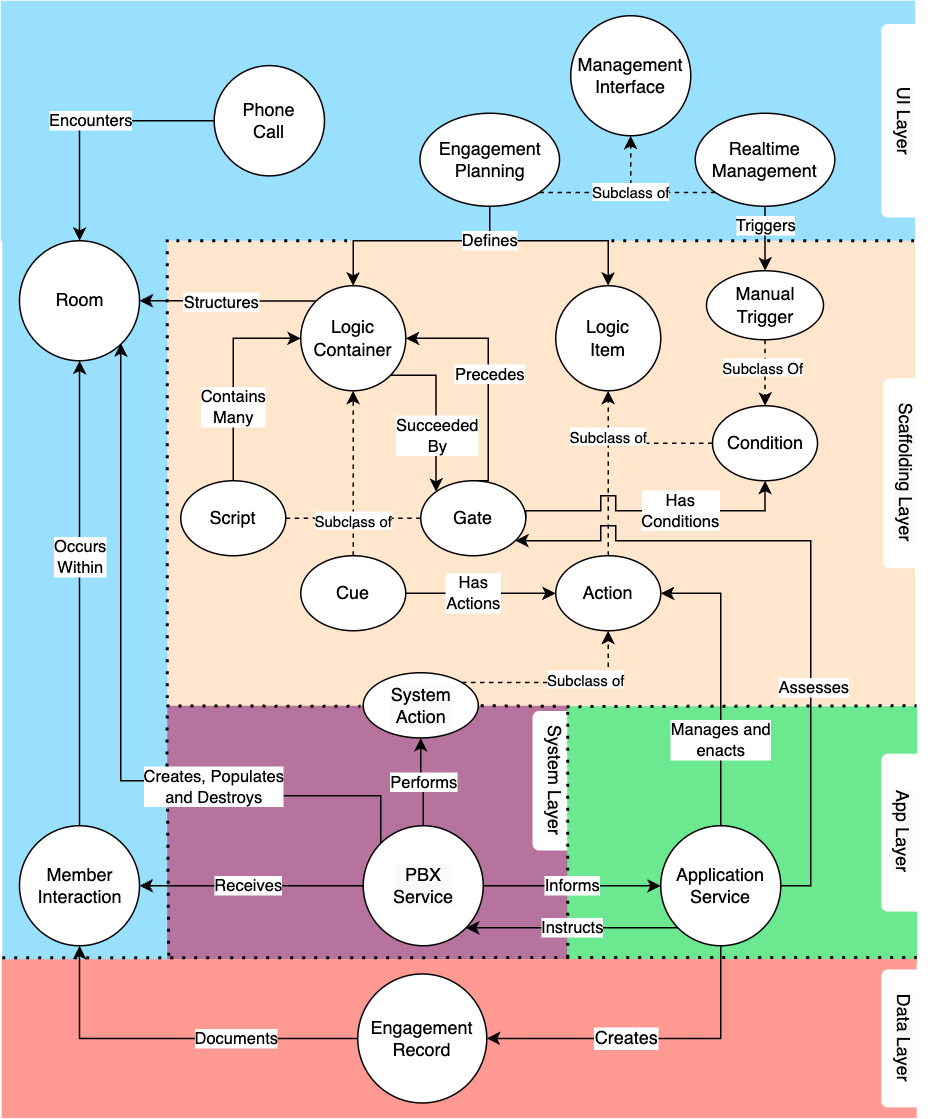
\includegraphics[width=0.8\columnwidth]{images/simplified.drawio.png}
  \caption{A visualisation of the classes and their relationships within \ONT{}, abbreviated for clarity and space. Solid arrows represent object properties (relationships). Circles depict classes whose parent classes are not shown (all are descendants from \textit{foaf} or \textit{sioc} classes). Ovals represent subclasses, connected to their parent class by dashed arrows (e.g. SystemAction is a subclass of Action).}
  \Description{A diagram giving an overview of most of the classes in \ONT{}, with labelled arrows representing relationships between classes. It is broken into five coloured layers. The first layer is blue, labelled as the "UI Layer", and contains six classes: Management interface, its subclasses Engagement Planning and Realtime Management, Phone Call, Room, and Member Interaction. Phone call encounters room. Member Interactions occur within Rooms. The next layer, the "Scaffolding Layer", is beige. It contains two parent classes: Logic container and logic item. Both are labelled as being defined by the Engagement Planning interface in the UI Layer. Logic container structures Rooms in the UI layer, and has 3 subclasses: Script, Cue and Gate. A script can contain many Logic Containers. A logic container is succeeded by a Gate, and Gates precede Logic Containers. Logic Item has two subclasses: Action and Condition. A Cue has actions, a gate has conditions. Condition has a single shown subclass, Manual Trigger, which is triggered by the Realtime Management interface in the UI Layer. Action has one shown subclass, System Action. The next layer, in green, is the "App Layer", which has one class: Application Service. Application Service assesses Gates, and manages and enacts Actions. The fourth layer is the purple "System Layer", which contains the PBX Service class. This receives Member Interactions from the UI layer, informs and receives instructions from the Application Service in the App Layer, and performs System Actions from the Scaffolding Layer. The final layer is the red "Data Layer", which contains the Engagement Record class. Engagement Records are created by the Application Service in the App Layer, and describe Member Interactions in the UI layer. }\label{fig:drawio}
\end{figure*}

Made up of relatively few classes, \ONT{} is designed to describe and structure the design space of synchronous group telephony engagement platforms, whilst still remaining abstract enough to encourage exploration, interpretation and expansion (addressing NFR2). To address NFR1, the ontology can be conceptualised as being made up of five layers of components: \textit{UI}, which describes how users and hosts interact with the system through phone calls and visual applications; \textit{Scaffolding}, which defines the components that, when combined, create the logic to orchestrates different engagement formats; \textit{System}, which describes the software (such as FreeSWITCH) by which the phone calls are initiated and manipulated; \textit{App}, which manages and enacts the Scaffolding logic and directs the System layer components;  and \textit{Data}, which refers to the data created, stored and retrieved by the App layer. 

To address NFR3, two forms of visual representation were also developed: one to communicate the relationships between the different layers of components of the ontology (Figure \ref{fig:drawio}); and the \ONT{} visual design vocabulary, which aims to support designers in designing, communicating, and understanding the technical requirements of different types of group engagements over synchronous telephony (an example is given in Figure \ref{fig:preshow}). For the sake of clarity and brevity, these diagrams exclude the base-level \textit{foaf} and \textit{sioc} axioms. The full class hierarchy is visible in Figure \ref{fig:hierarchy}. 

This section will give a detailed overview of the \ONT{} ontology, using these visuals as a communication aid.

\begin{figure}[h]
  \centering
  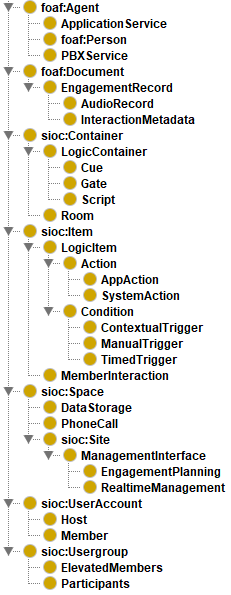
\includegraphics[width=0.25\linewidth]{images/hierarchy.png}
  \caption{Hierarchy of the classes utilised by \ONT{}, as displayed in the OWL development application Prot\'{e}g\'{e}.}
  \Description{A screenshot of the application Prot\'{e}g\'{e}, showing the list of classes within \ONT{}. Under foaf:Agent are Application Service, foaf:Person, and PBX Service. Under foaf:Document is Engagement Record, which has the subclasses Audio Record and Interaction Metadata. Under sioc:Container is Logic Container and Room. Logic Container has three subclasses: Cue, Gate and Script. Under sioc:Item is Member Interaction, Action, and Condition. Action has the subclasses App Action and System Action. Condition has the subclasses Contextual Trigger, Manual Trigger, and Timed Trigger. Under sioc:Space are Data Storage, Phone Call and sioc:Site. sioc:Site has Management Interface as a subclass, which also contains Engagement Planning and Realtime Management. sioc:UserAccount has the subclasses Host and Member. sioc:UserGroup has the subclasses Elevated Members and Participants.}
  \label{fig:hierarchy}
\end{figure}

\subsection{The UI Layer}

The UI Layer describes users and the methods by which they interact with the system---be that by a phone call or through a visual interface. Users (instances of \textit{foaf:Person}) interacting with the system are either a Host or Member (subclasses of \textit{sioc:UserAccount}). Note that while we have designed \ONT{} around interactions over standard phone calls, it's possible to apply these same concepts through other synchronous communication formats, such as WebRTC\footnote{https://webrtc.org/}---especially for Hosts, who will likely have access to an online interface.

Members are regular participants, and engage with the system through PhoneCalls (extends \textit{sioc:Space}). Through PhoneCalls, they encounter the system by populating audio spaces referred to as Rooms (extends \textit{sioc:Container}). Prior platforms only utilised a single Room, where all users were in a single conference call, but (as discussed later) multiple could be created simultaneously. MemberInteractions (extending \textit{sioc:Item}) occur inside these rooms, and could be utterances of speech or button presses. 

Hosts can access the visual ManagementInterface (extends \textit{sioc:Site}), which has two implementations depending on the state of the call: EngagementPlanning if the call is yet to start, and RealtimeManagement if it has. As an example, the Android app in \cite{Kazakos2016} is a ManagementInterface, used during the call to keep track of which participants wanted to ask questions, and mute and unmute them as needed. 

\begin{figure}[h]
  \centering
  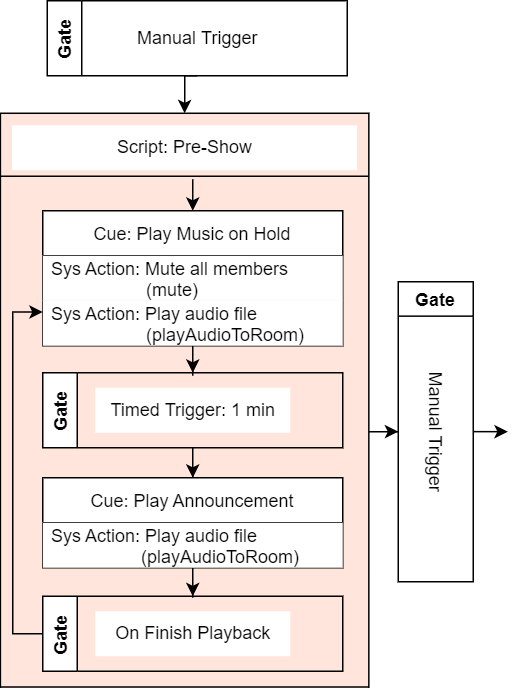
\includegraphics[width=0.4\columnwidth]{images/preshow.png}
  \caption{Using the visual design vocabulary to show how elements of the Scaffolding Layer can be configured to produce an automated pre-show routine. Here, the `Pre-Show' Script is initialised by the Host through a ManualTrigger. The Script contains four LogicContainers: two Gates and two Cues. The second Gate precedes the first Cue, forming a logic loop. This loop can be interrupted by the Host through a ManualTrigger, which would exit the Script.}~\label{fig:preshow}
  \Description{A flow chart style diagram showing how the vocabulary's components can be combined to create the logic for a pre-show routine. The first element in the flow is a Gate containing a Manual Trigger. This leads to a Script titled 'Pre-Show'. The first element inside the Script is a Cue titled 'Play Music on Hold'. It contains two Actions: 'Mute all members', which uses the mute System Action, and 'play audio file', which uses the 'play audio to room' System Action. Following this Cue is a Gate, with a Timed Trigger of one minute. Following the Gate is a second Cue, titled 'play announcement', containing one Action: 'play audio file', which uses the System Action 'play audio to room'. Following the Cue is a Gate with the Condition 'on finish playback'. The Gate then links back to the 'Play music on hold' Cue, forming a loop. The whole 'pre-show' Script is connected to another Gate with a Manual Trigger, which would interrupt the loop.}
\end{figure}

\subsection{The Scaffolding Layer}
The interplay of the components of the Scaffolding Layer creates the blueprints for different structured interactions (e.g. a Q\&A section, a breakout room session) during a call. These components are defined by the host through the EngagementPlanning interface. The permissions a participant has (e.g. if they can unmute themselves) can be controlled by assigning them to one of two subclasses of \textit{sioc:Usergroup}: ElevatedMembers or Participants (omitted from Figure \ref{fig:drawio} for space reasons). The remaining components are either LogicContainers (subclass of \textit{sioc:Container}) or LogicItems (subclass of \textit{sioc:Item}). LogicContainers contain LogicItems, and are assessed and enacted by the ApplicationService sequentially (similar to Twilio Studio). To support synchronous interactions and branching logic, multiple LogicContainers can be active at the same time (as demonstrated in Figure \ref{fig:talkshow}). A LogicContainer can be either a Script, Cue or Gate, whereas LogicItems are Actions or Conditions: 

\subsubsection{Condition (LogicItem)}

A small piece of logic relating to the call that can be evaluated to a Boolean (true or false) value. There are three main types of Conditions: TimedTriggers, which evaluate to true after a given length of time; ManualTriggers, which only become true through direct intervention by the host through the RealtimeManagement interface (e.g. the host presses a button to play an audio file); and ContextualTriggers, which can relate to particular factors within the call (e.g. `there are 10 participants present', `the audio file has finished playback'). ContextualTriggers are less formally defined in the vocabulary to support application-specific implementation.

\subsubsection{Action (LogicItem)}

An active intervention which can affect the flow of the call, managed by the ApplicationService in the Application Layer. Actions are one of two types: SystemActions and AppActions. SystemActions are performed in the System Layer as they directly interact with call audio or connections. They can be one of a limited set of interactions: \textit{dial}, \textit{hangup}, \textit{mute}, \textit{unmute}, \textit{transfer}, \textit{createRoom}, \textit{closeRoom}, \textit{playAudioToMember}, \textit{playAudioToRoom}, \textit{stopPlayback}, \textit{startRecording}, and \textit{stopRecording}. As with ContextualTriggers, AppActions are less strictly defined as they likely require per-application implementation within the ApplicationService. Examples include: `Mark participant Y as having raised their hand', `Move to the next agenda item', `Make participant X an ElevatedMember'.

The functionality required for an interaction's implementation can be identified by examining what LogicItems it uses: for example, listing the Conditions and Actions used in Figure \ref{fig:breakout} provides an answer to \textit{CQ1}.

\subsubsection{Gate (LogicContainer)}

Gates precede (and can succeed) other LogicContainers. They contain one or more Conditions connected by the logic operators AND or OR, and `unlock' once the ApplicationService in the System Layer evaluates the expression as true. For example: `The participant presses 8 AND the participant is muted'. Once the Gate is `unlocked', the LogicContainer it precedes becomes active. To support branching logic, multiple parallel Gates can be assessed simultaneously, each preceding a different LogicContainer (e.g. multiple options in an IVR menu: `\textit{press 1 to do X, press 2 to do Y}').  

\subsubsection{Cue (LogicContainer)}
Cues contain one or more Actions which are enacted when the preceding Gate is unlocked. If a succeeding Gate exists, it will start being assessed once the Cue's Actions have been initiated.

\subsubsection{Script (LogicContainer)}
Scripts contain other LogicContainers (including other Scripts) to support containerisation: allowing extended logic sequences to be initiated or interrupted by Gates. As an example, Figure \ref{fig:preshow} uses the visual design vocabulary to show a Script for a looping pre-show routine. In the routine, participants in the call are muted and music plays. After one minute, a pre-recorded announcement plays, and after it finishes the music plays again. As this Script is a LogicContainer with a succeeding Gate, the call's host can interrupt this loop at any time to start the show. If no loop is present, the final LogicContainer will exit the script upon completion (as seen in Figures \ref{fig:breakout} and \ref{fig:roundrobin}).

As will be demonstrated in Section \ref{section:scenarios}, through such combinations of Conditions, Gates, Actions, Cues, and Scripts, we can use \ONT{} to describe complex interactions.

\subsection{The Application Layer}

The Application Layer contains the ApplicationService: a software application (e.g. built using PHP, as in  \cite{Kazakos2016}) which puts the Scaffolding Layer into practice, assessing currently active Gates and managing any resulting Actions. It enacts all except SystemActions, which it instructs the System Layer (described below) to perform. The ApplicationService is a \textit{foaf:Agent}, as it is capable of programmatically taking independent action in response to changes in state.

\subsection{The System Layer}

The System Layer features the PBXService (also a \textit{foaf:Agent}): the key server-side component common to previous synchronous telephony platforms \cite{Kazakos2016, Talhouk2017, Yadav2017}. PBXService is an application capable of programmatically initiating and managing voice connections (e.g. via Voice Over IP, or the Public Switched Telephone Network) and creating, populating and destroying Rooms. FreeSWITCH is an example of a PBXService, and was used by Kazakos et al. in their project \cite{Kazakos2016}. Another popular example is Asterisk \footnote{https://www.asterisk.org/}. The PBXService enacts SystemActions and informs the ApplicationService of any changes in the call state, such as instances of MemberInteractions (e.g. buttons presses, vocal utterances, disconnections).

\subsection{The Data Layer}

The Data Layer concerns the storage of data, either for use within a call (e.g. playback of existing audio) or archiving. EngagementRecords (subclass of \textit{foaf:Document}) can either be AudioRecords or InteractionMetadata, and are created by the ApplicationService to document MemberInteractions. As an example of how these could be used, the process described in Figure \ref{fig:talkshow} could keep records of which Members raised their hands and which were unmuted---data which could be queried to answer \textit{CQ2}.
\section{Scaffolding Engagements through \ONT{}'s Design Vocabulary}
\label{section:scenarios}

This section will demonstrate the use the visual design vocabulary through the use of 3 scenarios, each featuring a different archetype of group interaction. As discussed previously, each features a use-case that was ideated during the development of \ONT{} as a way of creating and assessing functional requirements. The first scenario, the `talk show' format, demonstrates the applicability of \ONT{} to existing technology from prior work. The second, the `research workshop', acts as an example of how \ONT{} can be used to describe how current remote engagement practices (e.g. breakout rooms) can be implemented through telephony. The third, `speed dating' offers an exploration of how the same set of features can be reconfigured to support new, novel interactions with remote participants over the phone.

\subsection{Scenario 1: Talk Show}

\begin{figure}[h]
  \centering
  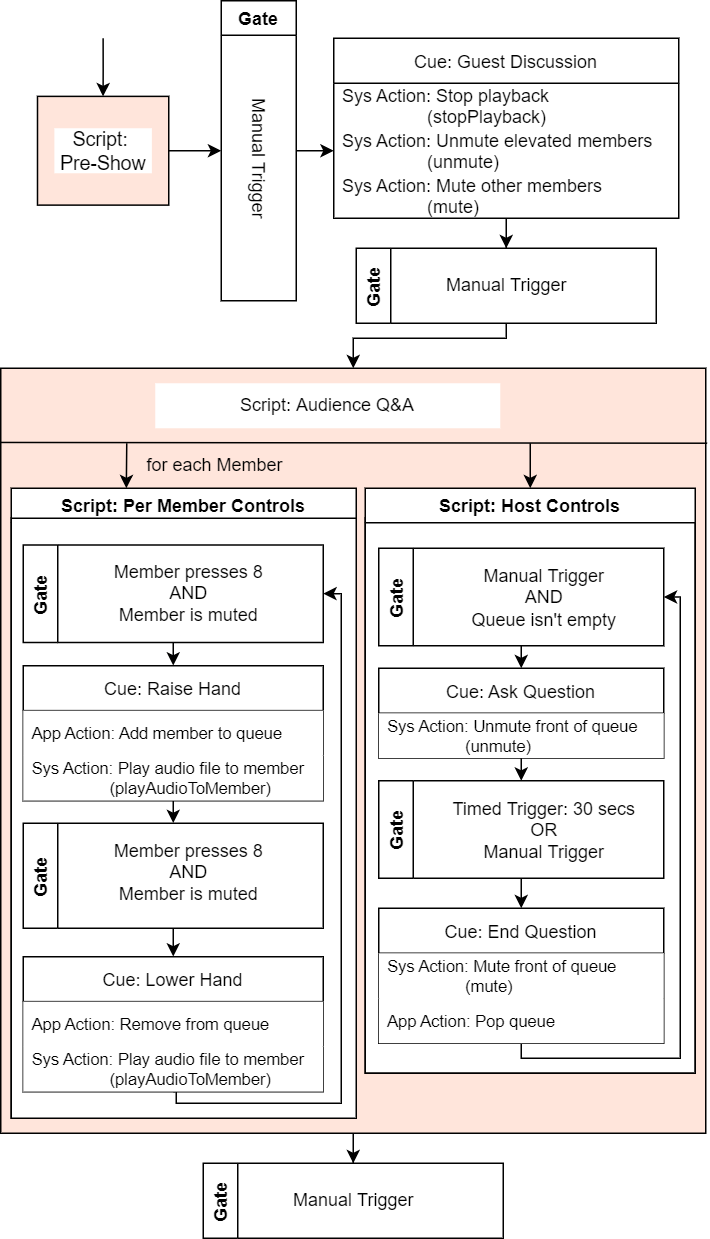
\includegraphics[width=0.5\columnwidth]{images/example_talkshow.drawio.png}
  \Description{Another flow chart style diagram, showing how a talk show could be implemented in \ONT{}. The first item is a Script labelled 'pre-show', referencing the previous diagram. This is followed by a Gate containing a Manual Trigger Condition. This is then followed by a Cue titled 'Guest Discussion', which has three System Actions: stop playback of playing audio files, unmute the elevated user group, and mute other members. This Cue is followed by another Gate with a Manual Trigger, which leads to another Script, titled 'Audience Q\&A'. This Script can be interrupted by a Manual Trigger, and contains two looping tracks of logic. The first, labelled 'for each member', features a Script titled 'per member controls'. The first item in this script is a Gate, with the conditions 'member presses 8' and 'member is muted', connected with the 'AND' operator. This gate is followed by a Cue titled 'raise hand', which has the App Action 'add member to queue' and a System Action 'play audio to member'. This is then followed by a Gate with the same conditions as before, which leads to a second cue titled 'lower hand'. This Cue has an App Action 'remove from queue' and another play audio to member System Action. It connects to the first Gate, forming a loop. The second track of logic in the parent 'Audience Q\&A' Script has a Script titled 'Host Controls'. This starts with a Gate containing a Manual Trigger and a 'queue isn't empty' contextual trigger, connected by the AND operator. This is followed by a Cue titled 'ask question', which has an unmute System Action labelled 'unmute front of queue'. This is then followed by another Gate, which has two conditions connected by the OR operator: a 30 seconds Timed Trigger, and a Manual Trigger. This Gate is followed by another Cue, titled 'end question', which contains a mute System Action ('mute front of queue') and an App Action ('pop queue'). This Cue is then connected to the first gate in the 'Host Controls' Script, forming a loop.}
  \caption{Using \ONT{} to prototype the interactions involved in a talk show with an audience Q\&A segment. The `Pre-Show' Script is detailed in Figure \ref{fig:preshow}. During the Q\&A, multiple Scripts are active at once: one for the Host, and one for each Member. Note that the handling of race conditions has been omitted to save space.}~\label{fig:talkshow}
\end{figure}

Figure \ref{fig:talkshow} shows how a talk show engagement format (described in Section \ref{section:talkshow}) with strict time-keeping can be scaffolded programmatically using \ONT{}. The main segments of the show (pre-show, guest discussion, and audience Q\&A) are transitioned between by the host through the use of Manual Triggers. The use of containerisation means that the `pre-show' Script previously shown in Figure \ref{fig:preshow} can be re-used. The `guest discussion' unmutes the Elevated Members group (i.e. the host and guests), and mutes everyone else. The `audience Q\&A' Script has two sets of asynchronous tracks: one which is used on a per-Member basis, letting callers add and remove themselves from the queue to ask questions through a button press; and one for the host to manage the queue. When triggered by the host, the Member at the front of the queue will be unmuted for 30 seconds (or manually interrupted by the host) to ask a question, before being muted again and removed from the queue. The Script is exited by a Manual Trigger, after which further logic could either end the show, or clear the queue and ensure that all participants are muted again before continuing. Planning the interaction through \ONT{} and observing used LogicItems shows that this system would need to implement mute, unmute, and audio playback SystemActions, as well as a queue system which can be manipulated by callers and the host.


\subsection{Scenario 2: Research Workshop}

\subsubsection{Overview}

Since the start of the COVID-19 pandemic, it has become more common to hold research workshops remotely though platforms such as Zoom: the `breakout room' feature (where callers can be temporarily subdivided into smaller discussion groups) can be used as an analogue for having separate tables of participants within a qualitative workshop to support group discussion and activities. This degree of dynamic manipulation of call topology has not yet been supported within existing synchronous group telephony platforms.

\begin{figure}[h]
  \centering
  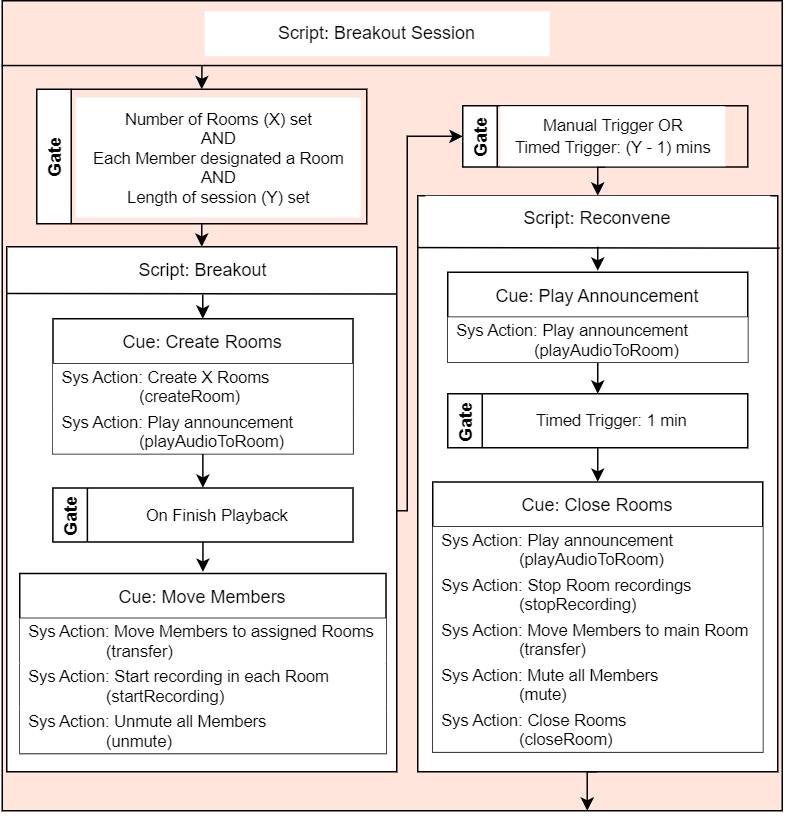
\includegraphics[width=0.5\columnwidth]{images/example_workshop.drawio.png}
  \Description{}
  \caption{Using \ONT{} to scaffold a `breakout room' interaction to be used during a distributed research workshop}~\label{fig:breakout}
  \Description{Another flow chart style diagram, showing how a breakout room interaction could be implemented in \ONT{} to facilitate a research workshop scenario. It consists of a 'Breakout Session' Script containing two gates and two nested scripts. It starts with a Gate with three conditions: 'number of rooms (X) set', 'each member designated a room', and 'length of session (Y)'; all connected with the 'AND' operator. Within these conditions, X and Y are previously set variables. This Gate is followed by a nested Script labelled 'Breakout', which starts with a Cue titled 'Create Rooms'. This cue has two System Actions: create X number of rooms and play announcement audio to the (main) room. This is followed by a Gate with the condition 'On Finish Playback', which connects to another Cue titled 'Move Members'. This Cue has three System Actions: move members to assigned rooms, start recording in each room, and unmute all members in the rooms. The 'Breakout' Script terminates with a Gate containing two conditions connected by the 'OR' operator: a Manual Trigger condition and a Y-1 minutes Timed Trigger (the length of session, Y, minus one minute). The Gate links to the next nested Script labelled 'Reconvene', which starts with a Cue titled 'Play Announcement'. This has one play audio to room System Action. This is followed by a Gate that contains a one minute Timed Trigger, followed by the final Cue within the 'Reconvene' Script titled 'Close Rooms'. The 'Close Rooms' Cue has five System Actions: play announcement audio to the rooms, stop room recordings, move members back to main room, mute all members, and close all (breakout) rooms. After completing the reconvene script, the parent breakout session script exits.}
\end{figure}

\subsubsection{\ONT{} Implementation}

Figure \ref{fig:breakout} shows how \ONT{} could be used to scaffold a `breakout' segment of a research workshop though synchronous telephony (answering \textit{CQ3}). Prior to commencing, this Script requires a configuration noting the number of Rooms to create, the length of time the breakout session should run for, and an assignment of which Members should go to each room. The Script will create the given number of Rooms, play a pre-recorded announcement to Members, and then move them to their assigned Room. The system records each room to a separate audio file for later reference by the researchers, who may not be present in all Rooms. When there is one minute left (or the Host intervenes) another announcement is played, and the Members are muted and moved back to the main Room when the timer expires. This interaction requires the PBXService to be able to create Rooms and assign Members to them: within FreeSWITCH (used by \cite{Kazakos2016, Talhouk2017, Yadav2017}), this can be achieved through the use of conferences\footnote{\url{https://freeswitch.org/confluence/display/FREESWITCH/mod\_conference}} and transfers\footnote{\url{https://freeswitch.org/confluence/display/FREESWITCH/mod\_dptools\%3A+transfer}}.


\subsection{Scenario 3: Speed dating}

\subsubsection{Overview}

Speed dating events typically involve a group of individuals being split into pairs to have short, one-on-one conversations, with pairs cycling every few minutes so that all suitably matched participants have a chance to meet. While fairly simple to organise in person, doing such structured interactions remotely through standard telephony would be highly labour intensive and prone to error: likely requiring participants manage their own timings and hold separate phone calls for each pairing.

\begin{figure}[h]
  \centering
  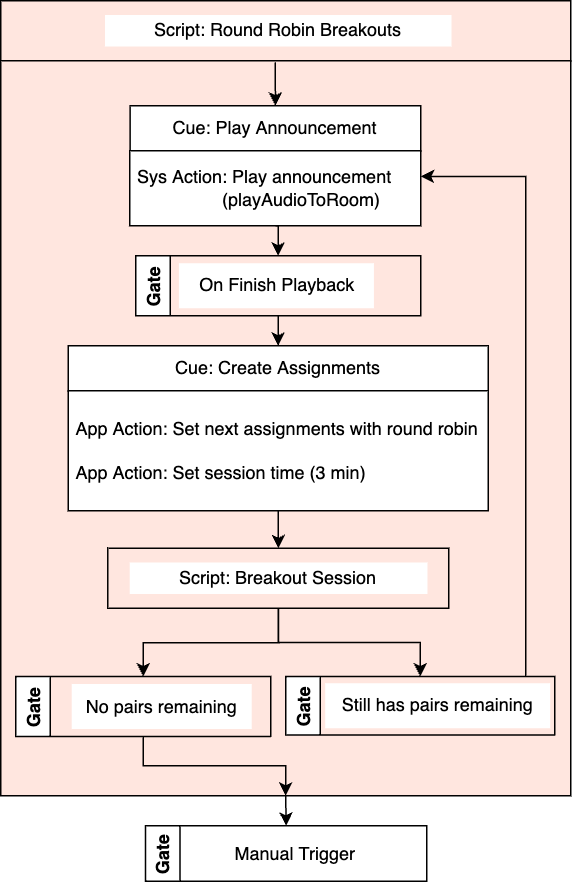
\includegraphics[width=0.4\columnwidth]{images/example_speeddating.drawio.png}
  \Description{}
  \caption{Using \ONT{} to scaffold a `speed dating' interaction using breakout rooms in a round robin configuration. The `Breakout Session' Script can be re-used from Figure \ref{fig:breakout} with minimal modification.}~\label{fig:roundrobin}
  \Description{Another flow chart, detailing a Script labelled 'Round Robin Breakouts'. The Script starts with a Cue titled 'Play Announcement' having one System Action: play announcement to the (main) room. The Cue is followed by a Gate with the condition 'On Finish Playback', which links to another Cue 'Create Assignments'. This Cue has two App Actions: set next assignments with round robin, and set session time (with a given example of 3 minutes). This followed by the previously discussed 'Breakout Session' Script, followed by two parallel Gates. The first contains the condition 'no pairs remaining', and leads to the end of the 'Round Robin Breakouts' Script. The other has the condition 'still has pairs remaining', and links back to the 'Play Announcement' Cue, forming a loop.}
\end{figure}

\subsubsection{\ONT{} Implementation}
Figure \ref{fig:roundrobin} shows the `speed dating' example, and demonstrates how programmatically manipulating the topology of meeting rooms opens up many new opportunities for remote interaction. This design uses the previous breakout room Script (altered to disable recording functionality) to facilitate the one-on-one conversations, with each pairing having their own Room. While the previous example relied on the Host manually assigning participants to groups, here the pairings would be assigned through the use of a round-robin algorithm\footnote{\url{https://en.wikipedia.org/wiki/Round-robin\_tournament}}, managed by the ApplicationService.
\section{Discussion}

% 1) how separating scaffolding, pbx and application makes development easier and more sustainable

\subsection{Supporting Design Exploration and Sustainability through Modularity}

A key feature of \ONT{} is its separation of a platform's component parts into five distinct layers: \textit{UI}, \textit{Scaffolding}, \textit{Application}, \textit{System} and \textit{Data}. By separating a synchronous telephony platform's implementation out into these layers, \ONT{} allows for the partial decoupling of the systems' key components from each other. A key benefit of this separation of concerns is reusability: different combinations of interactions can be implemented in the scaffolding layer, often without the need to update the rest of the system.

This separation is particularly beneficial to the System Layer: while PBXServices such as FreeSWITCH are freely available, installing and configuring them can be complicated and time consuming. 
Having such a limited number of SystemActions which can be performed by the PBXService provides the System Layer with a core feature-set: one which is unchanging between applications, but can be combined with logic from the Scaffolding and Application Layers to support a wide variety of interaction archetypes. For example, the research workshop and speed dating scenarios each re-used the same SystemActions (`\textit{createRoom}' and `\textit{transfer}') to produce markedly different experiences, without the need to change the PBXService. 

In contrast, existing synchronous group telephony platforms (as described in their publications) seem to have been explicitly designed to implement a single engagement format \cite{Kazakos2016, Talhouk2017, Yadav2019}. As such, the implementation of these platforms is tightly coupled to the `talk show' format, and implementing new interaction methods would require significant re-engineering.
While introducing new AppActions in \ONT{} will likely always require the development of additional features within the ApplicationService (e.g. the production of a queue system, or an implementation of round-robin), this can still be achieved without touching the PBXService: meaning that developers of such features don't necessarily need to deploy or have a technical understanding of complicated platforms like FreeSWITCH.
As a result, we argue that the reusability supported by an approach like \ONT{} results in a much lower barrier to the design and prototyping of platforms for synchronous group telephony.

% 2) enabling new types of synchronous IVR engagements through scaffolding

\subsection{Scaffolding New Interactions through Synchronous Group Telephony}

While the talk show format supported by previous synchronous telephony projects can be effective at delivering information to groups of participants, it offers limited opportunities for participant interaction and agency as, by necessity, participants spend most of the call muted. Not only is this incongruous with most participants' prior experiences of phone calls (which typically consist of unstructured discussion between two individuals), but it is also incompatible with any use-cases which require open discussion between participants, or for all participants (including the host) to be on equal footing. Despite these limitations, the use of alternatives to the talk show format within synchronous group telephony has not been adequately explored. As discussed, we believe that this is partially because prior platforms seem to have been designed around talk shows, and would require significant re-engineering to test new formats or be adapted in response to changing stakeholder requirements. However, we also posit that the lack of well defined and commonly agreed axioms can make designing, communicating, and visualising the processes of these engagement formats unwieldy.

We argue that the example scenarios presented in this paper using the visual vocabulary demonstrate that \ONT{} is flexible enough to support the exploration, development and communication of a wide variety of group interaction archetypes through synchronous telephony. The use of \ONT{} to scaffold a talk show format (Figure \ref{fig:talkshow}), complete with an automated pre-show routine (Figure \ref{fig:preshow}), demonstrates that it can be used to describe the engagements facilitated by existing synchronous group telephony platforms, and further highlights the value of a vocabulary which is able to describe and communicate these complex systems. Furthermore, during our experiences developing these scenarios through the design vocabulary there were multiple points where we had to consider unanticipated system requirements, or gaps in logic. For example, when defining the timed Gate to reconvene breakout groups (Figure \ref{fig:breakout}), we realised that there should be a manual override available to the host in case they wanted to reconvene the groups early. Such instances highlight that this format has value in being used for developing low-fidelity logical prototypes.

This paper has also demonstrated how the Scaffolding and App Layers can be used to produce new engagement models, beyond the capabilities of previous synchronous group telephony platforms. For example, while prior platforms limited participants to the largely passive role of an audience member, the research workshop example (Figure \ref{fig:breakout}) supports all participants engaging in open discussion through the use of breakout rooms, without requiring anyone to be muted. The speed dating example (Figure \ref{fig:roundrobin}) demonstrates how this could be taken further: by implementing the `round-robin' algorithm  in the ApplicationService to determine participant pairings, it demonstrated the potential for programmatic scaffolding to produce remote encounters where all participants have comparable levels of agency. This could be expanded even further to support highly structured engagement formats, such as Robert's Rules of Order: a parliamentary procedure used in many contexts to support group discussion and decision making with `\textit{due regard for every member's opinion}' \cite{robert2020}. In such a case, the ApplicationService acts as the arbiter of the engagement---able to direct proceedings, potentially with minimal intervention from the Host. 

Such possibilities suggest that synchronous telephony offers potential for facilitating group interactions beyond those covered in the scenarios presented in this paper. We argue that this potential can be more easily explored through \ONT{}: that the visual design vocabulary supports the design, communication, and analysis of a wide array of new engagement formats hitherto unutilised in remote contexts with offline participants.

% 3) using the layers to explore each as their own design space

\subsection{Accessing Under-Explored Design Spaces}

One of the key benefits of a common vocabulary is that it can be used to share an understanding of a domain which can be communicated across people, computers or both \cite{struder1998}. As \ONT{}'s design vocabulary is more approachable, less technical, and more easily communicable than the underlying architectures and systems it describes, it offers designers and engineers a bridge for discussion and exploration of the potential interactions offered by synchronous group telephony. Furthermore, as this visual format is grounded by a formal ontology, it opens a design space that can be referenced, shared, and built upon by different systems---independent from their underlying software stack. Such an approach lowers the barrier to entry to the exploration, experimentation and appropriation of the uses of synchronous group telephony in new engagement contexts and use cases.

The layered framing of \ONT{} also supports approaching each of these layers as their own design spaces, independent of the rest of the platform's infrastructure. The Data Layer provides a strong example: while explorations have been made regarding how systems can support participatory recordkeeping practices \cite{rolan2017}, the HCI community has performed little to no research into how organisations performing voice-based stakeholder engagements can (or should) approach recordkeeping practices. Researchers within this design space could explore how informed consent should be taken, recorded or rescinded through voice-based platforms; or how resulting audio records could be created, stored, accessed, documented, appraised, and disposed of through voice-based interfaces. Examples of what explorations could be made within the Application Layer include investigating how programmatic, agent-based systems (such as chatbots \cite{Jain2018, Yadav2019} or virtual participants \cite{Bartindale2021}) could be incorporated into the synchronous activities offered by these platforms. As such, we posit that the layers of \ONT{} are rich design spaces, within which we can explore how other practices and technologies can interact with the medium of synchronous group telephony.
\section{Future Work}

We are currently in the process of incorporating \ONT{} into a demonstrable synchronous telephony platform. Within our future work, we plan to use \ONT{} to support the kinds of group interaction formats illustrated in this paper's scenarios, explore some of the previously discussed recordkeeping concepts within the Data Layer, and investigate how \ONT{} could also be used to scaffold asynchronous interactions before, during and after synchronous engagements \cite{Yadav2017}. Through the implementation of this platform, we hope to be able to provide other researchers in this space recommendations for how to put \ONT{} into practice, as well as further refine the vocabulary in response to findings resulting from its implementation.

It is also worth noting that much of \ONT{} could be applied to other mediums, such as synchronous video, through digital standards such as WebRTC. We wished to focus on its application to group telephony within this paper, given that it is a particularly under-explored design space. However, as \ONT{} is a formal ontology, future work could extend it to suit other mediums.

\section{Conclusion}

Recent years have demonstrated the value and potential of synchronous telephony platforms which enable engagements with remote, offline groups of participants through traditional phone networks. However, this potential has been under-explored, with all published platforms in this space following the same `talk show' engagement format. In response, this paper presents \ONT{}: a design vocabulary, grounded in a formal ontology describing the components of a platform needed to support the dynamic scaffolding of group interactions through synchronous telephony. Demonstrating through a series of scenarios describing three different use cases of synchronous group telephony, we argue that \ONT{} is not only capable of describing the interactions enabled by previously published systems, but also new interaction formats with a flexibility previously unavailable within remote telephony. We argue that \ONT{} provides an approachable, structured vocabulary which offers a more sustainable framework for system design, and highlights that the layers of components within these systems each offer a rich, under-explored design space.

%% The acknowledgments section is defined using the "acks" environment
%% (and NOT an unnumbered section). This ensures the proper
%% identification of the section in the article metadata, and the
%% consistent spelling of the heading.
\begin{acks}

\end{acks}

%%
%% The next two lines define the bibliography style to be used, and
%% the bibliography file.
\bibliographystyle{ACM-Reference-Format}
\bibliography{references}


\end{document}
\endinput

